\documentclass{article}
\usepackage[utf8]{inputenc}
\usepackage{listings}
\usepackage{multimedia} % to embed movies in the PDF file
\usepackage{graphicx}
\usepackage{comment}
\usepackage[english]{babel}
\usepackage{amsmath}
\usepackage{amsfonts}
\usepackage{subfigure}
\usepackage{wrapfig}
\usepackage{multirow}
\usepackage{verbatim}

\newtheorem{theorem}{Theorem}[section]
\newtheorem{lemma}[theorem]{Lemma}
\newtheorem{corollary}[theorem]{Corollary}
%\newtheorem{algorithm}[theorem]{Algorithm}
\newtheorem{remark}[theorem]{Remark}
\newenvironment{proof}{\noindent {\bf Proof:} }{\hfill $\Box$ \\[2ex] }
\newenvironment{keywords}{\begin{quote} {\bf Key words} }
                         {\end{quote} }
\newenvironment{AMS}{\begin{quote} {\bf AMS subject classifications} }
                         {\end{quote} }


\newcommand{\eref}[1]{\mbox{\rm(\ref{#1})}}
\newcommand{\tref}[1]{\mbox{\rm\ref{#1}}}
\newcommand{\set}[2]{\left\{ #1 \; : \; #2 \right\} }
\newcommand{\deq}{\raisebox{0pt}[1ex][0pt]{$\stackrel{\scriptscriptstyle{\rm def}}{{}={}}$}}

\newcommand {\DS} {\displaystyle}

\newcommand{\real}{\mathbb{R}}
\newcommand{\compl}{\mathbb{C}}



\newcommand {\half} {\mbox{$\frac{1}{2}$}}
\newcommand{\force}{{\mathbf{f}}}
\newcommand{\strain}{{\boldsymbol{\varepsilon}}}
\newcommand{\stress}{{\boldsymbol{\sigma}}}
\renewcommand{\div}{{\boldsymbol{\nabla}}}

\newcommand {\cA} {{\cal A}}
\newcommand {\cB} {{\cal B}}
\newcommand {\cC} {{\cal C}}
\newcommand {\cD} {{\cal D}}
\newcommand {\cE} {{\cal E}}
\newcommand {\cL} {{\cal L}}
\newcommand {\cP} {{\cal P}}
\newcommand {\cQ} {{\cal Q}}
\newcommand {\cR} {{\cal R}}
\newcommand {\cV} {{\cal V}}
\newcommand {\cW} {{\cal W}}
\newcommand {\CH} {{\cal H}}
\newcommand {\CS} {{\cal S}}


\newcommand{\bzero}{\mathbf{0}}
\newcommand{\ba}{\mathbf{a}}
\newcommand{\bb}{\mathbf{b}}
\newcommand{\bc}{\mathbf{c}}
\newcommand{\bd}{\mathbf{d}}
\newcommand{\be}{\mathbf{e}}
\newcommand{\bff}{\mathbf{f}}
\newcommand{\bg}{\mathbf{g}}
\newcommand{\bh}{\mathbf{h}}
\newcommand{\bn}{\mathbf{n}}
\newcommand{\bp}{\mathbf{p}}
\newcommand{\bq}{\mathbf{q}}
\newcommand{\br}{\mathbf{r}}
\newcommand{\bs}{\mathbf{s}}
\newcommand{\bt}{\mathbf{t}}
\newcommand{\bu}{\mathbf{u}}
\newcommand{\bv}{\mathbf{v}}
\newcommand{\bw}{\mathbf{w}}
\newcommand{\bx}{\mathbf{x}}
\newcommand{\by}{\mathbf{y}}
\newcommand{\bz}{\mathbf{z}}
\newcommand{\bA}{\mathbf{A}}
\newcommand{\bB}{\mathbf{B}}
\newcommand{\bC}{\mathbf{C}}
\newcommand{\bD}{\mathbf{D}}
\newcommand{\bE}{\mathbf{E}}
\newcommand{\bF}{\mathbf{F}}
\newcommand{\bG}{\mathbf{G}}
\newcommand{\bH}{\mathbf{H}}
\newcommand{\bI}{\mathbf{I}}
\newcommand{\bJ}{\mathbf{J}}
\newcommand{\bK}{\mathbf{K}}
\newcommand{\bL}{\mathbf{L}}
\newcommand{\bM}{\mathbf{M}}
\newcommand{\bN}{\mathbf{N}}
\newcommand{\bO}{\mathbf{O}}
\newcommand{\bP}{\mathbf{P}}
\newcommand{\bQ}{\mathbf{Q}}
\newcommand{\bR}{\mathbf{R}}
\newcommand{\bS}{\mathbf{S}}
\newcommand{\bU}{\mathbf{U}}
\newcommand{\bV}{\mathbf{V}}
\newcommand{\bW}{\mathbf{W}}
\newcommand{\bX}{\mathbf{X}}
\newcommand{\bY}{\mathbf{Y}}
\newcommand{\bZ}{\mathbf{Z}}

\newcommand{\cO}{ {\cal O} }
\newcommand{\CT}{ {\cal T} }
\newcommand{\IL}{{\mathbb L}}
\newcommand{\sIL}{{{{\mathbb L}_s}}}
\newcommand{\bOmega}{{\boldsymbol{\Omega}}}
\newcommand{\bPsi}{{\boldsymbol{\Psi}}}

\newcommand{\bgamma}{{\boldsymbol{\gamma}}}
\newcommand{\bmu}{{\boldsymbol{\mu}}}
\newcommand{\blambda}{{\boldsymbol{\lambda}}}
\newcommand{\bLambda}{{\boldsymbol{\Lambda}}}
\newcommand{\bpi}{{\boldsymbol{\pi}}}
\newcommand{\bPi}{{\boldsymbol{\Pi}}}
\newcommand{\bphi}{{\boldsymbol{\phi}}}
\newcommand{\bPhi}{{\boldsymbol{\Phi}}}
\newcommand{\bpsi}{{\boldsymbol{\psi}}}
\newcommand{\btheta}{{\boldsymbol{\theta}}}
\newcommand{\bTheta}{{\boldsymbol{\Theta}}}
\newcommand{\bSigma}{{\boldsymbol{\Sigma}}}
\newcommand{\sump}{\sideset{}{^{'}}\sum} 
\DeclareMathOperator*{\Res}{Res}
\DeclareMathOperator{\OO}{O}
\DeclareMathOperator{\oo}{o}
\DeclareMathOperator{\erfc}{erfc}
\def\Xint#1{\mathchoice
   {\XXint\displaystyle\textstyle{#1}}%
   {\XXint\textstyle\scriptstyle{#1}}%
   {\XXint\scriptstyle\scriptscriptstyle{#1}}%
   {\XXint\scriptscriptstyle\scriptscriptstyle{#1}}%
   \!\int}
\def\XXint#1#2#3{{\setbox0=\hbox{$#1{#2#3}{\int}$}
     \vcenter{\hbox{$#2#3$}}\kern-.5\wd0}}
\def\ddashint{\Xint=}
\def\pvint{\Xint-}






\title{AMATH 568 Homework 8}
\author{Cade Ballew \#2120804}
\date{March 4, 2022}

\begin{document}
	
\maketitle
	
\section{Problem 1}
Considering the BVP 
  \begin{align*}
    \begin{cases} \epsilon y''(x) + \sin(x) y'(x) + \sin(2x) y(x) = 0,\\
      y(0) = \pi,\\
      y(\pi) = 0, \end{cases}
  \end{align*}
we expect to see a boundary layer near $x=0$, because $\sin x>0$ arbitrarily close to $x=0$ (and on the entire interval $(0,\pi)$). Thus, the function for our outer layer is defined by taking $\epsilon=0$ and solving
  \begin{align*}
    \begin{cases}\sin(x) y_{\text{out}}'(x) + \sin(2x) y_{\text{out}}(x) = 0,\\
      y_{\text{out}}(\pi) = 0. \end{cases}
  \end{align*}
Solving this with an integrating factor,
\begin{align*}
y_{\text{out}}(x)=C\exp\left(-\int_0^x\frac{\sin 2s}{\sin s}ds\right)=C\exp\left(-\int_0^x2\cos s ds\right)=Ce^{-2\sin x}.
\end{align*}
Plugging in our boundary condition, we get that $C=0$, so we conclude that 
\[
y_{\text{out}}=0.
\]
Now, we look to find the inner expansion by considering a substitution $z=\frac{x}{\delta(\epsilon)}$ and defining $Y_{\text{in}}(z)=y(\delta z)$. Then, our differential equation becomes 
\[
\frac{\epsilon}{\delta^2}Y''_{\text{in}}(z)+\frac{\sin (\delta z)}{\delta}Y'_{\text{in}}(z)+\sin(2\delta z)Y_{\text{in}}(z)=0.
\]
Now, we Taylor expand the sine function around $z_0=0$ to get
\[
\frac{\epsilon}{\delta^2}Y''_{\text{in}}(z)+\frac{1}{\delta}(\delta z+\OO(\delta^3))Y'_{\text{in}}(z)+(2\delta z+\OO(\delta^3))Y_{\text{in}}(z)=0.
\]
To find a dominant balance, we note that the second term will always have a lower order term than the third, so we need to balance the first and second terms. To do this, we need $\frac{\epsilon}{\delta^2}=1$, so we take $\delta=\sqrt{\epsilon}$ and an expansion for $Y_{\text{in}}$ is given by 
\[
Y_{\text{in}}\sim\sum_{n=0}^\infty Y_n\epsilon^{n/2}.
\]
Looking at the leading order, $Y_0$ must satisfy the BVP
  \begin{align*}
    \begin{cases}  Y_0''(z) + z Y_0'(z) = 0,\\
      Y_0(0) = \pi. 
      \end{cases}
  \end{align*}
We can see that 
\[
Y_0'(z)=c_1e^{-z^2/2} 
\]
satisfies this equation. Then,
\begin{align*}
Y_0(z)=c_1\int e^{-z^2/2}dz+c_2=\sqrt{\frac{\pi}{2}}c_1\erf\left(\frac{z}{\sqrt{2}}\right)+c_2=C\erf\left(\frac{z}{\sqrt{2}}\right)+c_2
\end{align*}
where $C$ and $c_2$ are constants. Noting that $\erf0=0$, our boundary condition gives $c_2=\pi$, so,
\[
Y_{\text{in}}(z)=C\erf\left(\frac{z}{\sqrt{2}}\right)+\pi+\OO(\epsilon^{1/2}).
\]
Now, we find the constant $C$ by applying the matching condition at the bottom of page 336 in the text. Namely, we need that to leading order
\[
\lim_{z\to\infty,z>0}Y_{\text{in}}(z)=\lim_{x\to0,x>0}y_{\text{out}}(x).
\]
Noting that $\erf x\to1$ as $x\to\infty$, this condition becomes $C+\pi=0$, so we get that $C=-\pi$. Now, $y_{\text{out}}$ and $Y_{\text{in}}$ agree in the matching region 
\[
0\ll\frac{x}{\sqrt{\epsilon}}\ll\epsilon^{-1/2},
\]
and the matching term in this region is given by 
\[
\lim_{z\to\infty,z>0}Y_{\text{in}}(z)=\lim_{x\to0,x>0}y_{\text{out}}(x)=0.
\]
Combining everything, our lowest-order uniform approximation to the BVP is
\[
y(x;\epsilon)=Y_{\text{in}}(x/\sqrt{\epsilon})+y_{\text{out}}(x)-y_{\text{match}}=-\pi\erf\left(\frac{x}{\sqrt{2\epsilon}}\right)+\pi.
\]
  
\section{Problem 2}
\subsection{Part a}
Now, consider the BVP 
\begin{align*}
    \begin{cases} \epsilon y_1''(x) + x y_1'(x) = x \cos(x),\\
      y_1(-1) = 2,\\
      y_1(0) = c_1. \end{cases}
  \end{align*}
We expect a boundary layer near 0, because $x<0$ on the interval $(-1,0)$. Thus, the function for our outer layer is given by taking $\epsilon=0$ and solving
\begin{align*}
    \begin{cases} x y_{\text{out}}'(x) = x \cos(x),\\
      y_{\text{out}}(-1) = 2. \end{cases}
  \end{align*}
This gives that $y_{\text{out}}'(x)=\cos x$, so 
\[
y_{\text{out}}(x)=\sin x+C.
\]
Incorporating our boundary condition, $2=\sin(-1)+C$, so $C=2-\sin(-1)=2+\sin1$. Thus,
\[
y_{\text{out}}(x)=\sin x+2+\sin1.
\]
Now, we look to find the inner expansion by considering a substitution $z=\frac{x}{\delta(\epsilon)}$ and defining $Y_{\text{in}}(z)=y(\delta z)$. Then, our differential equation becomes 
\[
\frac{\epsilon}{\delta^2}Y''_{\text{in}}(z)+\frac{\delta z}{\delta}Y'_{\text{in}}(z)=\delta z\cos{\delta z}.
\]
Taylor expanding the RHS at $z_0=0$,
\[
\frac{\epsilon}{\delta^2}Y''_{\text{in}}(z)+zY'_{\text{in}}(z)=\delta z(\delta z+\OO(\delta^3)).
\]
To find a dominant balance, we need to balance the first two terms, meaning that $\frac{\epsilon}{\delta^2}=1$, so $\delta=\sqrt{\epsilon}$. Then, 
\[
Y''_{\text{in}}(z)+zY'_{\text{in}}(z)=\epsilon z^2+\OO(\epsilon^2),
\]
so an expansion for $Y_{\text{in}}$ is given by 
\[
Y_{\text{in}}\sim\sum_{n=0}^\infty Y_n\epsilon^{n/2}.
\]
To leading order, we must then have that 
\begin{align*}
    \begin{cases} Y_0''(z)+zY_0'(z) = 0,\\
      Y_0(0) = c_1. \end{cases}
  \end{align*}
From problem 1, we know that a general solution is given by
\[
Y_0(z)=C\erf\left(\frac{z}{\sqrt{2}}\right)+C',
\]
and plugging in our boundary condition gives that $C'=c_1$, so
\[
Y_0(z)=C\erf\left(\frac{z}{\sqrt{2}}\right)+c_1.
\]
Now, we find the constant $C$ by applying the matching condition at the bottom of page 336 in the text (noting that our interval is negative instead of positive). Namely, we need that to leading order
\[
\lim_{z\to-\infty,z<0}Y_{\text{in}}(z)=\lim_{x\to0,x<0}y_{\text{out}}(x).
\]
Noting that $\erf x\to-1$ as $x\to-\infty$, this condition becomes $-C+c_1=2+\sin1$, so $C=-(2+\sin1-c_1)$. Thus, 
\[
Y_{\text{in}}\sim -(2+\sin1-c_1)\erf\left(\frac{z}{\sqrt{2}}\right)+c_1+\OO(\epsilon^{1/2}).
\]
Now, $y_{\text{out}}$ and $Y_{\text{in}}$ agree in the matching region 
\[
0\ll\frac{x}{\sqrt{\epsilon}}\ll\epsilon^{-1/2},
\]
and the matching term in this region is given by 
\[
{y}_{\text{match}}=\lim_{z\to-\infty,z<0}Y_{\text{in}}(z)=\lim_{x\to0,x<0}y_{\text{out}}(x)=2+\sin1.
\]
Combining everything, our lowest-order uniform approximation to the BVP is
\begin{align*}
y(x;\epsilon)&=Y_{\text{in}}(x/\sqrt{\epsilon})+y_{\text{out}}(x)-y_{\text{match}}\\&=\sin x+2+\sin1-(2+\sin1-c_1)\erf\left(\frac{x}{\sqrt{2\epsilon}}\right)+c_1-(2+\sin1)\\&=
\sin x-(2+\sin1-c_1)\erf\left(\frac{x}{\sqrt{2\epsilon}}\right)+c_1.
\end{align*}

\subsection{Part b}
Now, consider the BVP 
\begin{align*}
    \begin{cases} \epsilon y_2''(x) + x y_2'(x) = x \cos(x),\\
      y_2(1) = 2,\\
      y_2(0) = c_1. \end{cases}
  \end{align*}
We expect a boundary layer near 0, because $x>0$ on the interval $(0,1)$. Thus, the function for our outer layer is given by taking $\epsilon=0$ and solving
\begin{align*}
    \begin{cases} x y_{\text{out}}'(x) = x \cos(x),\\
      y_{\text{out}}(1) = 2. \end{cases}
  \end{align*}
This gives that $y_{\text{out}}'(x)=\cos x$, so 
\[
y_{\text{out}}(x)=\sin x+C.
\]
Incorporating our boundary condition, $2=\sin1+C$, so $C=2-\sin1$. Thus,
\[
y_{\text{out}}(x)=\sin x+2-\sin1.
\]
Now, we look to find the inner expansion by considering a substitution $z=\frac{x}{\delta(\epsilon)}$ and defining $Y_{\text{in}}(z)=y(\delta z)$. Then, our differential equation becomes 
\[
\frac{\epsilon}{\delta^2}Y''_{\text{in}}(z)+\frac{\delta z}{\delta}Y'_{\text{in}}(z)=\delta z\cos{\delta z}.
\]
Taylor expanding the RHS at $z_0=0$,
\[
\frac{\epsilon}{\delta^2}Y''_{\text{in}}(z)+zY'_{\text{in}}(z)=\delta z(\delta z+\OO(\delta^3)).
\]
To find a dominant balance, we need to balance the first two terms, meaning that $\frac{\epsilon}{\delta^2}=1$, so $\delta=\sqrt{\epsilon}$. Then, 
\[
Y''_{\text{in}}(z)+zY'_{\text{in}}(z)=\epsilon z^2+\OO(\epsilon^2),
\]
so an expansion for $Y_{\text{in}}$ is given by 
\[
Y_{\text{in}}\sim\sum_{n=0}^\infty Y_n\epsilon^{n/2}.
\]
To leading order, we must then have that 
\begin{align*}
    \begin{cases} Y_0''(z)+zY_0'(z) = 0,\\
      Y_0(0) = c_2. \end{cases}
  \end{align*}
From problem 1, we know that a general solution is given by
\[
Y_0(z)=C\erf\left(\frac{z}{\sqrt{2}}\right)+C',
\]
and plugging in our boundary condition gives that $C'=c_1$, so
\[
Y_0(z)=C\erf\left(\frac{z}{\sqrt{2}}\right)+c_2.
\]
Now, we find the constant $C$ by applying the matching condition at the bottom of page 336 in the text. Namely, we need that to leading order
\[
\lim_{z\to\infty,z>0}Y_{\text{in}}(z)=\lim_{x\to0,x>0}y_{\text{out}}(x).
\]
Noting that $\erf x\to1$ as $x\to\infty$, this condition becomes $C+c_2=2-\sin1$, so $C=2-\sin1-c_2$. Thus, to leading order
\[
Y_{\text{in}}\sim (2-\sin1-c_2)\erf\left(\frac{z}{\sqrt{2}}\right)+c_2.
\]
Now, $y_{\text{out}}$ and $Y_{\text{in}}$ agree in the matching region 
\[
0\ll\frac{x}{\sqrt{\epsilon}}\ll\epsilon^{-1/2},
\]
and the matching term in this region is given by 
\[
y_{\text{match}}=\lim_{z\to\infty,z>0}Y_{\text{in}}(z)=\lim_{x\to0,x>0}y_{\text{out}}(x)=2-\sin1.
\]
Combining everything, our lowest-order uniform approximation to the BVP is
\begin{align*}
y_2(x;\epsilon)&=Y_{\text{in}}(x/\sqrt{\epsilon})+y_{\text{out}}(x)-y_{\text{match}}\\&=\sin x+2-\sin1+(2-\sin1-c_2)\erf\left(\frac{x}{\sqrt{2\epsilon}}\right)+c_2-(2-\sin1)\\&=
\sin x+(2-\sin1-c_2)\erf\left(\frac{x}{\sqrt{2\epsilon}}\right)+c_2.
\end{align*}

\subsection{Part c}
Now, we wish to solve the BVP 
\begin{align*}
    \begin{cases} \epsilon y''(x) + x y'(x) = x \cos(x),\\
      y(1) = 2,\\
      y(-1) = 2. \end{cases}
  \end{align*}
by combining our solutions from parts a and b. To do this, we set $c_1=c_2$ and enforce that our functions are identical on our new extended domain. Combining these,
\[
\sin x-(2+\sin1-c_1)\erf\left(\frac{x}{\sqrt{2\epsilon}}\right)+c_1=\sin x+(2-\sin1-c_1)\erf\left(\frac{x}{\sqrt{2\epsilon}}\right)+c_1
\]
which gives that $-2-\sin1+c_1=2-\sin1-c_1$, so $c_1=c_2=2$. Thus, we can plug this in for $y_1$ and $y_2$ to find that a uniform approximation of the combined BVP is given by
\[
y(x;\epsilon)=\sin x-\sin1\erf\left(\frac{x}{\sqrt{2\epsilon}}\right)+2.
\]
Plotting this in Desmos for $\epsilon = 0.1, 0.05, 0.01$, we observe the following. \\
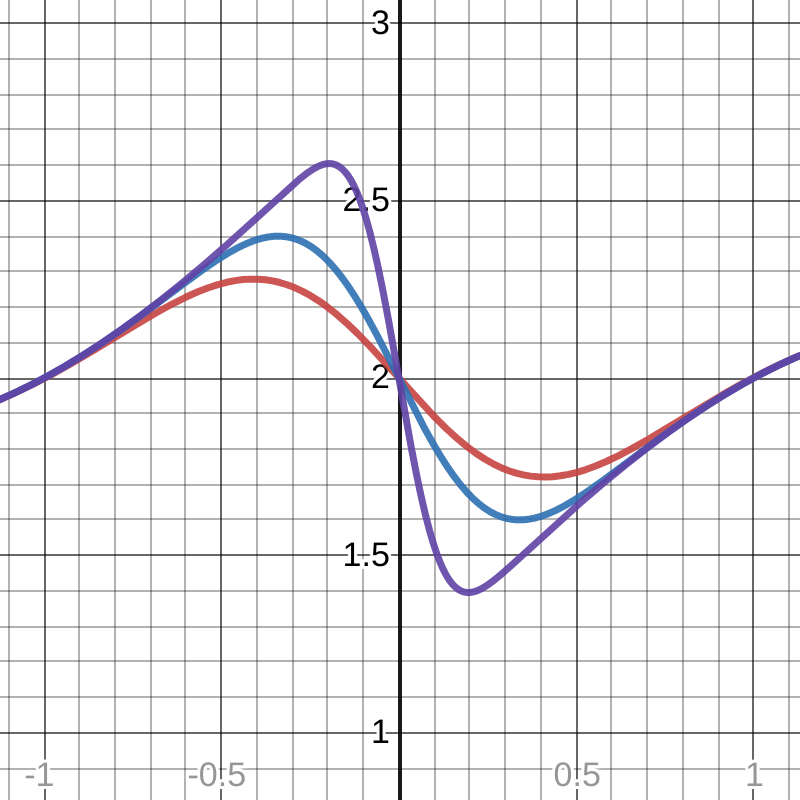
\includegraphics[scale=0.5]{desmos-graph.png}\\
where the red plot is $\epsilon=0.1$, the blue plot is $\epsilon=0.05$, and the purple plot is $\epsilon=0.01$.
\end{document}
